\documentclass[man]{apa6}

\usepackage{amssymb,amsmath}
\usepackage{ifxetex,ifluatex}
\usepackage{fixltx2e} % provides \textsubscript
\ifnum 0\ifxetex 1\fi\ifluatex 1\fi=0 % if pdftex
  \usepackage[T1]{fontenc}
  \usepackage[utf8]{inputenc}
\else % if luatex or xelatex
  \ifxetex
    \usepackage{mathspec}
    \usepackage{xltxtra,xunicode}
  \else
    \usepackage{fontspec}
  \fi
  \defaultfontfeatures{Mapping=tex-text,Scale=MatchLowercase}
  \newcommand{\euro}{€}
\fi
% use upquote if available, for straight quotes in verbatim environments
\IfFileExists{upquote.sty}{\usepackage{upquote}}{}
% use microtype if available
\IfFileExists{microtype.sty}{\usepackage{microtype}}{}

% Table formatting
\usepackage{longtable, booktabs}
\usepackage{lscape}
% \usepackage[counterclockwise]{rotating}   % Landscape page setup for large tables
\usepackage{multirow}		% Table styling
\usepackage{tabularx}		% Control Column width
\usepackage[flushleft]{threeparttable}	% Allows for three part tables with a specified notes section
\usepackage{threeparttablex}            % Lets threeparttable work with longtable

% Create new environments so endfloat can handle them
% \newenvironment{ltable}
%   {\begin{landscape}\begin{center}\begin{threeparttable}}
%   {\end{threeparttable}\end{center}\end{landscape}}

\newenvironment{lltable}
  {\begin{landscape}\begin{center}\begin{ThreePartTable}}
  {\end{ThreePartTable}\end{center}\end{landscape}}

  \usepackage{ifthen} % Only add declarations when endfloat package is loaded
  \ifthenelse{\equal{\string man}{\string man}}{%
   \DeclareDelayedFloatFlavor{ThreePartTable}{table} % Make endfloat play with longtable
   % \DeclareDelayedFloatFlavor{ltable}{table} % Make endfloat play with lscape
   \DeclareDelayedFloatFlavor{lltable}{table} % Make endfloat play with lscape & longtable
  }{}%



% The following enables adjusting longtable caption width to table width
% Solution found at http://golatex.de/longtable-mit-caption-so-breit-wie-die-tabelle-t15767.html
\makeatletter
\newcommand\LastLTentrywidth{1em}
\newlength\longtablewidth
\setlength{\longtablewidth}{1in}
\newcommand\getlongtablewidth{%
 \begingroup
  \ifcsname LT@\roman{LT@tables}\endcsname
  \global\longtablewidth=0pt
  \renewcommand\LT@entry[2]{\global\advance\longtablewidth by ##2\relax\gdef\LastLTentrywidth{##2}}%
  \@nameuse{LT@\roman{LT@tables}}%
  \fi
\endgroup}


  \usepackage{graphicx}
  \makeatletter
  \def\maxwidth{\ifdim\Gin@nat@width>\linewidth\linewidth\else\Gin@nat@width\fi}
  \def\maxheight{\ifdim\Gin@nat@height>\textheight\textheight\else\Gin@nat@height\fi}
  \makeatother
  % Scale images if necessary, so that they will not overflow the page
  % margins by default, and it is still possible to overwrite the defaults
  % using explicit options in \includegraphics[width, height, ...]{}
  \setkeys{Gin}{width=\maxwidth,height=\maxheight,keepaspectratio}
\ifxetex
  \usepackage[setpagesize=false, % page size defined by xetex
              unicode=false, % unicode breaks when used with xetex
              xetex]{hyperref}
\else
  \usepackage[unicode=true]{hyperref}
\fi
\hypersetup{breaklinks=true,
            pdfauthor={},
            pdftitle={Child language experience in a Tseltal Mayan village},
            colorlinks=true,
            citecolor=blue,
            urlcolor=blue,
            linkcolor=black,
            pdfborder={0 0 0}}
\urlstyle{same}  % don't use monospace font for urls

\setlength{\parindent}{0pt}
%\setlength{\parskip}{0pt plus 0pt minus 0pt}

\setlength{\emergencystretch}{3em}  % prevent overfull lines


% Manuscript styling
\captionsetup{font=singlespacing,justification=justified}
\usepackage{csquotes}
\usepackage{upgreek}

 % Line numbering
  \usepackage{lineno}
  \linenumbers


\usepackage{tikz} % Variable definition to generate author note

% fix for \tightlist problem in pandoc 1.14
\providecommand{\tightlist}{%
  \setlength{\itemsep}{0pt}\setlength{\parskip}{0pt}}

% Essential manuscript parts
  \title{Child language experience in a Tseltal Mayan village}

  \shorttitle{Child language experience in a Tseltal Mayan village}


  \author{Marisa Casillas\textsuperscript{1}, Penelope Brown\textsuperscript{1}, \& Stephen C. Levinson\textsuperscript{1}}

  % \def\affdep{{"", "", ""}}%
  % \def\affcity{{"", "", ""}}%

  \affiliation{
    \vspace{0.5cm}
          \textsuperscript{1} Max Planck Institute for Psycholinguistics  }

  \authornote{
    Correspondence concerning this article should be addressed to Marisa
    Casillas, Wundtlaan 1, 6525 XD Nijmegen, The Netherlands. E-mail:
    \href{mailto:Marisa.Casillas@mpi.nl}{\nolinkurl{Marisa.Casillas@mpi.nl}}
  }


  \abstract{Enter abstract here. Each new line herein must be indented, like this
line.}
  \keywords{keywords \\

    \indent Word count: X
  }





\usepackage{amsthm}
\newtheorem{theorem}{Theorem}[section]
\newtheorem{lemma}{Lemma}[section]
\theoremstyle{definition}
\newtheorem{definition}{Definition}[section]
\newtheorem{corollary}{Corollary}[section]
\newtheorem{proposition}{Proposition}[section]
\theoremstyle{definition}
\newtheorem{example}{Example}[section]
\theoremstyle{definition}
\newtheorem{exercise}{Exercise}[section]
\theoremstyle{remark}
\newtheorem*{remark}{Remark}
\newtheorem*{solution}{Solution}
\begin{document}

\maketitle

\setcounter{secnumdepth}{0}



\section{Introduction}\label{introduction}

Much of developmental language science revolves around one central
question: what linguistic evidence (i.e., what types and how much) is
needed to support first language acquisition? Early claims about
children's language environments characterized linguistic `input' as
syntactically complex and error-prone, with no negative evidence (REFS).
However, decades of work has overturned this view entirely: the speech
that children hear and use in their interactions with others is rich
with multimodal information that children can leverage to infer
linguistic knowledge. In fact, children's own speech productions appear
to closely mirror the stochastic patterns in their linguistic input
(REFS), convincingly accounting for the kinds of errors children do and
don't make in spontaneous speech (REFS; see also REFS for similar work
regarding phonological learning).

In the last two decades, the role of children's linguistic environments
on their language development has become a topic of intense focus in
developmental psychology, with studies showing repeatedly that the
amount of child-directed speech (CDS) children hear influences their
language development, particularly their vocabulary (REFS). For example,
{[}TO DO: Fill in later{]}. Some studies have also linked the quantity
of directed speech children hear to their speed of lexical retrieval and
their syntactic development (REFS; Weisleder; LuCiD; Huttenlocher).
{[}TO DO: Fill in later after reading Huttenlocher{]}. Child-directed
speech estimates have traditionally come from short at-home or in-lab
video recordings of caregiver-child interaction. But recently many
researchers have also used daylong audio recordings (e.g., with the
LENA(C) system) to track the approximate amount of spoken language in
children's at-home language environments; tracking information about how
much of the talk is child-directed by annotating sub-samples of the
recording (REFS; Weisleder) or looking at other cues to interactional
behavior (REFS; Romeo).

The conclusion drawn in much of this work is that child-directed speech
is the ideal register for learning words; especially for
\emph{referential} word learning (i.e., concrete nouns and verbs; REFS).
In line with this idea, experimental studies have conclusively shown
that infant-directed speech is nearly universally preferred over
adult-directed speech by young children (REFS ManyBabies, etc.). Perhaps
more importantly, child-directed speech is often produced under
conditions of joint activity, in which caregivers and children
coordinate their behavior in order to accomplish interactional goals
(e.g., daily routines of feeding, diaper changing, and play). Using
head-mounted eyetrackers, Chen Yu and colleagues (REFS) have
demonstrated that coordination during object-play exchanges {[}TO DO:
Fill in later{]}. Crucially, then, estimates of child-directed speech
quantity may functionally predict children's word learning because they
index the frequency with which children engage in rich, multimodal
interactions with their caregivers; interactions in which children can
actively and contingently elicit just the right linguistic information
at just the right time to be optimally interesting and useful for
learning (REFS; Eve's paper on homophonic Vs in French). There are,
however, at least two major caveats to this body of work relating CDS
quantity and language development.

First, while there is overwhelming evidence linking CDS quantity to
vocabulary size, links to grammatical development are much more scant
(REFS: Huttenlocher; others???). Learning a language involves mastery of
its systemic underpinnings, e.g., its phonology, morphology, and syntax.
While there is clear reason for CDS to have referentially more clear
speech--which is good for learning concrete vocabulary---it's less
obvious that the ability to learn syntactic structures is similarly
facilitated {[}TO DO: Start with Yurovsky paper + refrences therein{]}.
On the other hand, many usage-based approaches to language development
and processing (e.g., REFS) suggest that much of our syntactic knowledge
is wrapped up in lexically specified representations; what is good for
the lexicon may also be good for syntax. Taken together with
Huttenlocher's findings, the relationship between CDS and syntactic
development may be less linear (i.e., more exposure != more skill) and
more like {[}TO DO: fill in{]}.

Second, findings regarding the importance of CDS quantity for language
development have typically only focused on Western (primarily North
American) populations (e.g., REFS), fundamentally limiting our ability
to generalize the effects to children acquiring language worldwide
(REFS: WEIRD). While there is certainly insight to be gained by looking
at within-population variation, researchers are more likely to find the
places where their assumptions break down when they study child language
development in new populations. Ethnographic work with traditional
non-Western communities has demonstrated that caregiver-child
interaction styles vary immensely from place to place, with some reports
of little or no child-directed speech (\emph{Table 1}; Gaskins, 2006;
Lieven, 1994??). Although some of these children hear very little CDS,
there are no reports of significant delay in their linguistic
development. On the contrary, children in these communities are reported
to acquire language with `typical'-looking benchmarks: they tend to
start pointing (REFS: Liszkowski) and talking (REFS: Rogoff et al.,
2003?; Brown??) around the same time we would expect for Western
middle-class infants. However, it is difficult to make direct
comparisons between these ethnographic reports and reports from Western
settings that use entirely different methods of sampling and analysis.
To our knowledge, only a handful of researcherers have attempted to
quantitatively describe the language environments of children growing up
in traditional non-Western communities. We briefly highlight two recent
efforts.

Scaff, Cristia, and colleagues (REFS: 2017; in preparation) have used a
number of different data collection methods to estimate how much speech
children hear in an indigenous Tsimane community in Bolivia.
Collectively, their results suggest that Tsimane children NN or fewer
minutes {[}TO DO: \textless{}\textless{} fill in numbers{]} of CDS per
hour. For comparison, children from Western middle-class homes are
reported to hear between NN and NN minutes of CDS per hour {[}TO DO:
\textless{}\textless{} fill in numbers{]} (REFS: Alex's paper + the refs
therein, but also the newer Tamis-LeMonda paper; maybe give estimates w/
age ranges for each??), with children in working-class homes hearing
between NN and NN minutes of CDS per hour {[}TO DO:
\textless{}\textless{} fill in numbers{]}.

Laura Shneidman and colleagues (REFS; 2010; 2012) analyzed speech from
1-hour at-home video recordings of Yucatec Mayan children and American
children between 13 and 35 months. Shneidman and Goldin-Meadow's (REFS;
2012) analyses of the video recordings yielded four main findings:
compared to the American children, (a) the Mayan children heard many
fewer utterances per hour, (b) a much smaller proportion of the
utterances they heard were \emph{child-directed}, (c) the proportion of
child-directed utterances increased dramatically with age, matching
American children's by 35 months, and that (d) most of the added CDS
came from other children (e.g., older siblings and cousins). They also
demonstrated that the lexical diversity of CDS children heard at 24
months---particularly from adult speakers---predicted their vocabulary
knowledge at 35 months.

These groundbreaking studies on Tsimane and Yucatec Mayan children's
early language environments lead us to a number of important interim
conclusions. First, children in each of these communities appear able to
acquire their languages with relatively little CDS. Second, the
frequency with which they are addressed increases with age. Third, other
children may be the primary source of CDS in similar communities. And
finally, despite these differences, CDS from adults may still be the
most robust predictor of vocabulary growth.

\subsection{The current study}\label{the-current-study}

\begin{itemize}
\tightlist
\item
  In this paper we examine the linguistic experiences of 10 Tseltal
  Mayan children. Why Mayan?
\item
  Non-WEIRD
\item
  Rich area of research: Little CDS from report---potentially a great
  case for looking at a functioning acquisition system with minimal
  environmental input
\item
  Many linguistically and culturally similar communities for comparison
  (see Shneidman, Pye, etc.)
\item
  See slides for more
\item
  A major contribution of this work is to use daylong recordings, which
  allow us to estimate\ldots{} (TLM paper on short vs.~longer recs).

  \begin{itemize}
  \tightlist
  \item
    At the same time, there is potentially great value in knowing about
    what happens during interactional bursts when they happen, so we
    track \ldots{} tt and va as well
  \end{itemize}
\item
  Our aim is to develop a child language environment profile for Tseltal
  Mayan, one that gives an impression of the speech children hear around
  them and the type of speech that is addressed to them directly. 
\end{itemize}

\begin{itemize}
\tightlist
\item
  Results:
\item
  How much speech do children hear overall and what proportion of that
  is directed to them? How does that compare to other communities we've
  studied?

  \begin{itemize}
  \tightlist
  \item
    \emph{measures}: XDS and TDS minutes per hour and proportion (from
    random selections only)
  \end{itemize}
\item
  How do ADS and TDS differ?

  \begin{itemize}
  \tightlist
  \item
    \emph{measures}: utt length, repetitiveness, F0 peaks and ranges,
    questions, imperatives (?)
  \end{itemize}
\item
  How much speech do children hear during bouts/bursts of interaction?
  How often do these bursts occur?

  \begin{itemize}
  \tightlist
  \item
    \emph{measures}: deltas for m/h TDS, \#utts TDS, \# TT transitions
    between random, tt, and va: are they actually different?
  \item
    \emph{measures}: XDS and TDS minutes per hour and proportion (from
    tt and va selections: do they show similar age effects?)
  \item
    \emph{measures}: sliding window in random to match mean TDS rate/TT
    transition rates
  \end{itemize}
\item
  Does interaction influence linguistic practice?

  \begin{itemize}
  \tightlist
  \item
    \emph{measures}: m/h CHI vocs, \# CHI vocs, \& voc mat between
    random, tt, and va
  \end{itemize}
\item
  Discussion
\item
  Summary of findings
\item
  When thinking about quantity: Do we care about the avg over the day or
  do bursts matter more?

  \begin{itemize}
  \tightlist
  \item
    Benefits of naps between bursts? Natural input cycle? How many
    \enquote{good} minutes are enough to spur learning on?
  \end{itemize}
\item
  How should we think about CDS? What is universal about its format?
\item
  So what is the impact of input in this community? What do we predict?

  \begin{itemize}
  \tightlist
  \item
    One point often raised: do these kids show a delay? Problematize
    this.
  \item
    More interesting: language experience itself shapes use of
    mechanisms for learning, e.g., learning fro overhearing (Shneidman)
  \end{itemize}
\item
  Big issue we have to face as work continues in this vein: what are
  these kids learning? We can't continue to pretend that we are capable
  of defining and encapsulating a phenomenon as emergent as language.
\item
  Limitations

  \begin{itemize}
  \tightlist
  \item
    no video data
  \item
    only 10 kids
  \end{itemize}
\end{itemize}

\section{Methods}\label{methods}

\subsection{How to define temporal contingency for turn
taking}\label{how-to-define-temporal-contingency-for-turn-taking}

Many other studies of child-caregiver turn taking use an arbitrary
cut-off for detecting contingency (5 seconds?? Look up references). We
base ours on measures of turn taking in interactions with infants and
young children. Hilbrink et al. (2015) looked at interaction in a
longitudinal corpus from 3 to 18 months and found that infants'
responses to mothers began between -700ms and 1200ms relative to the end
of the mothers' turns. Complementarily, mothers' responses to infant
vocalizations began between -350ms and 650ms relative to the end of the
infants' turns. Casillas et al. (2016) investigated the timing of
question-answer responses from caregiver to child and from child to
caregiver with children between 20 and 35 months. In their study,
children's responses typically started between -500ms and 650ms relative
to the end of their caregivers' turns. Caregivers' responses typically
started between -1000ms and 400ms relative to the end of their
children's turns. Because both studies focused on fairly intensive bouts
of interaction, and both within WEIRD parental contexts, we defined
contingent responses in the current data with slightly generous
allowances for overlap and gap: contingent responses must begin with no
more than 1000ms of overlap and 2000ms of gap relative to the offset of
the first speaker's turn. We used this same criteria for finding
child-to-other turn transitions and other-to-child turn transitions.
Transitions were only counted if the other speaker's turn was coded as
addressed to \enquote{T} (the target child).

\subsection{Participants}\label{participants}

\subsection{Material}\label{material}

\subsection{Procedure}\label{procedure}

\subsection{Data analysis}\label{data-analysis}

\section{Results}\label{results}

\subsection{Still to graph}\label{still-to-graph}

3: sliding window in random to match mean TDS rate/TT transition rates
4: utt length, repetitiveness, F0 peaks and ranges

\subsection{SHOULD I ADD DATAPOINTS ON THE UPH FIGS TO SHOW SHNEIDMAN'S
DATA?}\label{should-i-add-datapoints-on-the-uph-figs-to-show-shneidmans-data}

Age 1: - US: CDS 616 (SD=231); ADS/OCDS 278 (SD=247) -- 79\% XDS from
MOT (\textasciitilde{}60\% XDS MOT is CDS); 8\% XDS from children
(mostly ADS/OCDS) - Mayan: CDS 86 (SD=59); ADS/OCDS 342 (SD=201) -- 31\%
XDS from MOT (\textasciitilde{}4\% XDS MOT is CDS); 60\% XDS from
children (\textasciitilde{}50\% XDS other kids was ADS/OCDS) Age18mo?:
Age 2: - US: CDS M=815, SD=376; ADS/OCDS M=411, SD=318 -- M=65\%,
SD=28\% from MOT (directed: M=800, SD=381; overheard: M=211, SD =55); --
M=7\%, SD=10\% from kids (directed: M=15, SD=22; overheard: M=86,
SD=141) - Mayan: CDS M=274, SD=166; ADS/OCDS M=271, SD=136 -- M=19\%,
SD=17\% from MOT (directed:M=104, SD=100; overheard:M=82 SD=52); --
M=61\%, SD=27\% from kids (directed:M=104, SD=100; overheard:M=82 SD=52)
Age35mo?

\subsubsection{Observation only data}\label{observation-only-data}

13 months Directed speech 140 (55); Overheard speech 377 (176) 18 months
Directed speech 211 (70); Overheard speech 240 (96) 24 months Directed
speech 315 (69); Overheard speech 360 (73) (I think these data weren't
coded for adult vs.~child speaker)

\begin{figure}
\centering
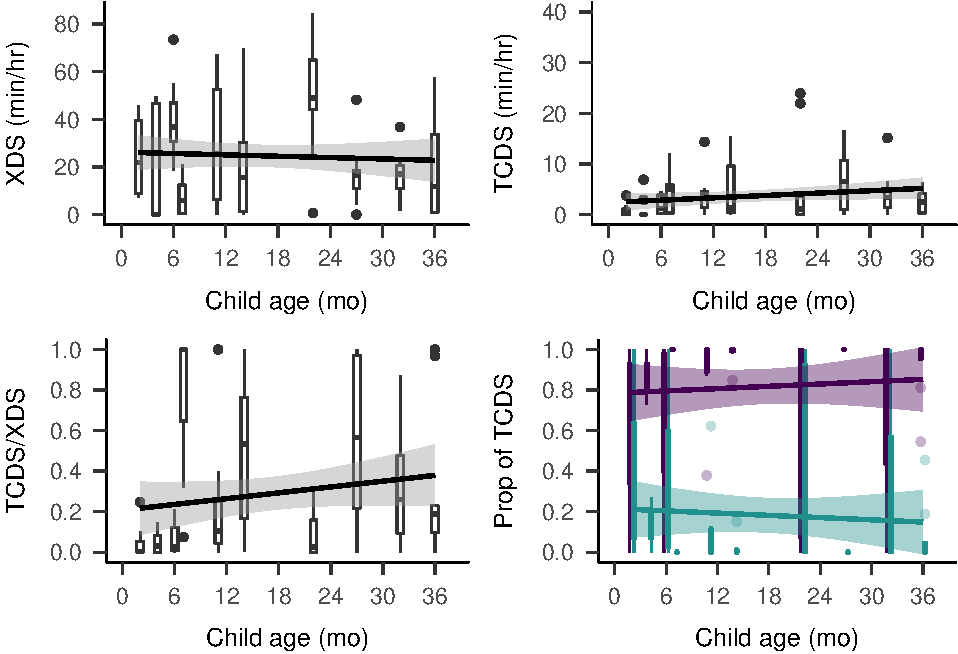
\includegraphics{Tseltal-CLE_files/figure-latex/plot_XDS_TDS_quantity_random-1.pdf}
\caption{}
\end{figure}

\begin{figure}
\centering
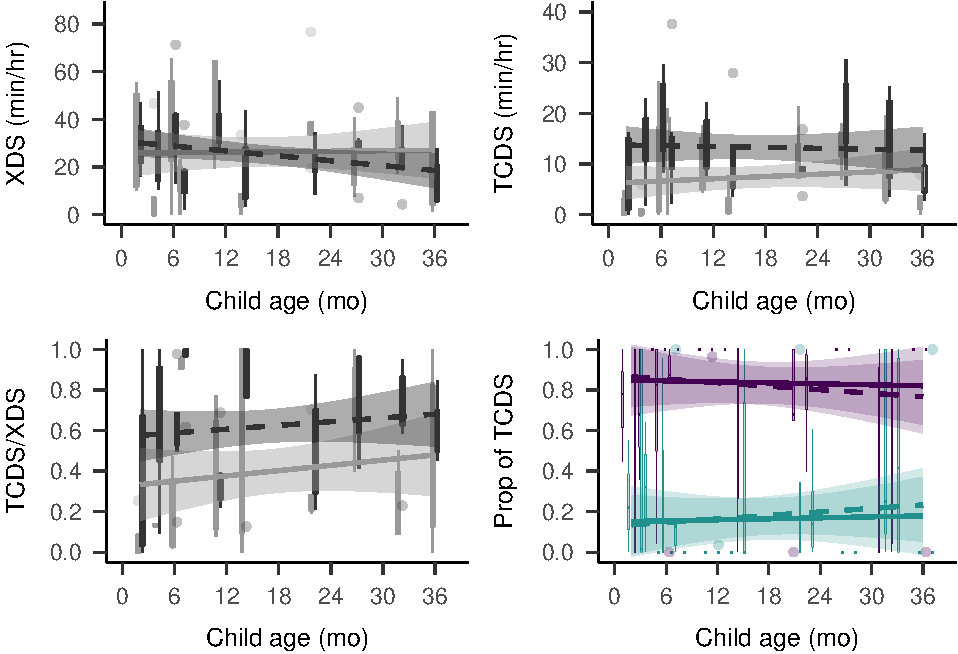
\includegraphics{Tseltal-CLE_files/figure-latex/plot_XDS_TDS_quantity_nonrandom-1.pdf}
\caption{}
\end{figure}

\begin{figure}
\centering
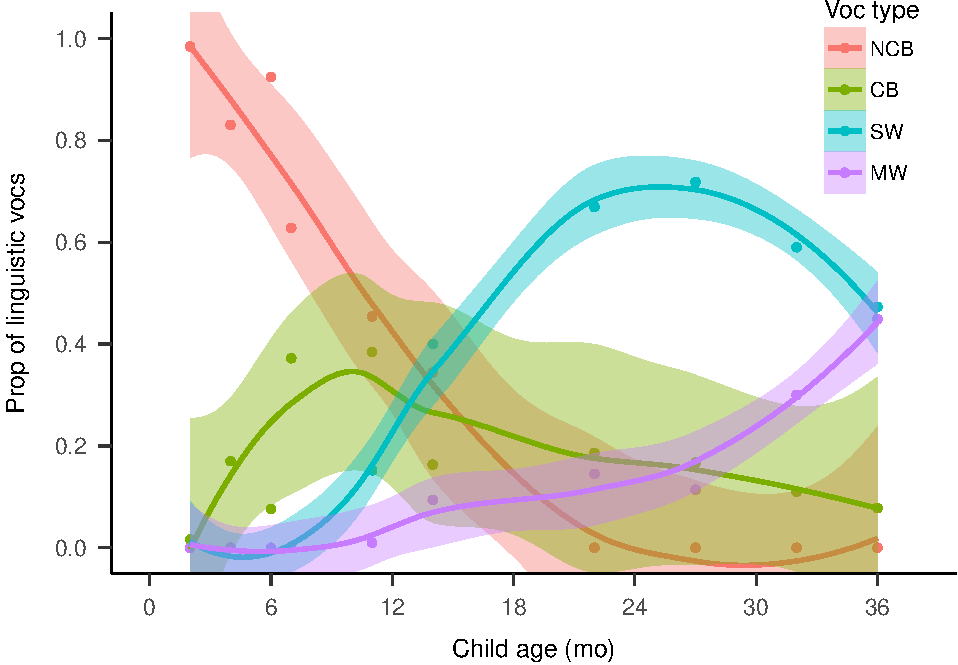
\includegraphics{Tseltal-CLE_files/figure-latex/plot_chi_voctypes_overall-1.pdf}
\caption{}
\end{figure}

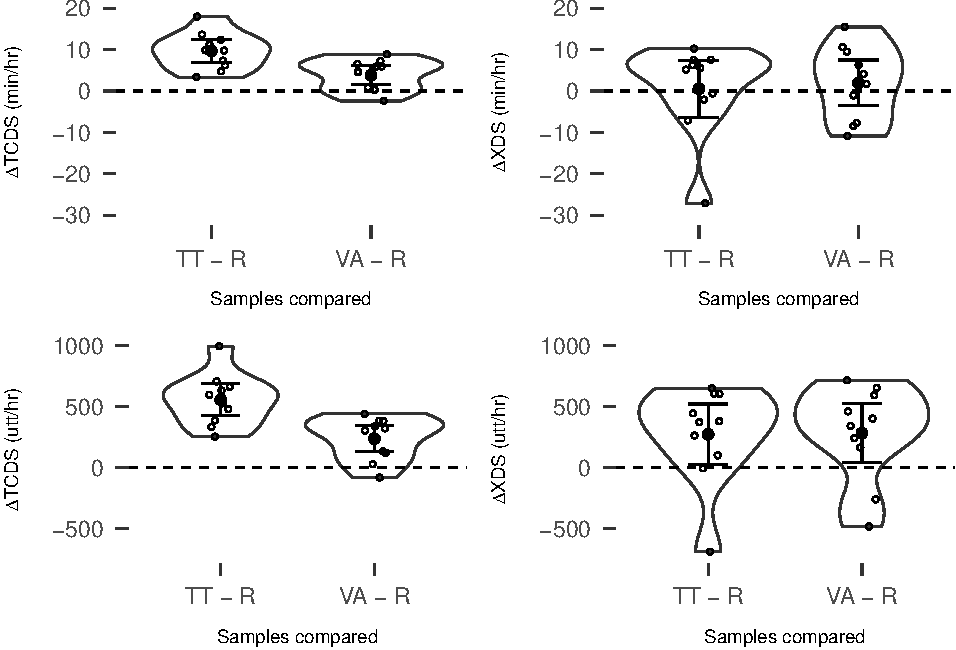
\includegraphics{Tseltal-CLE_files/figure-latex/plot_sample_differences-1.pdf}
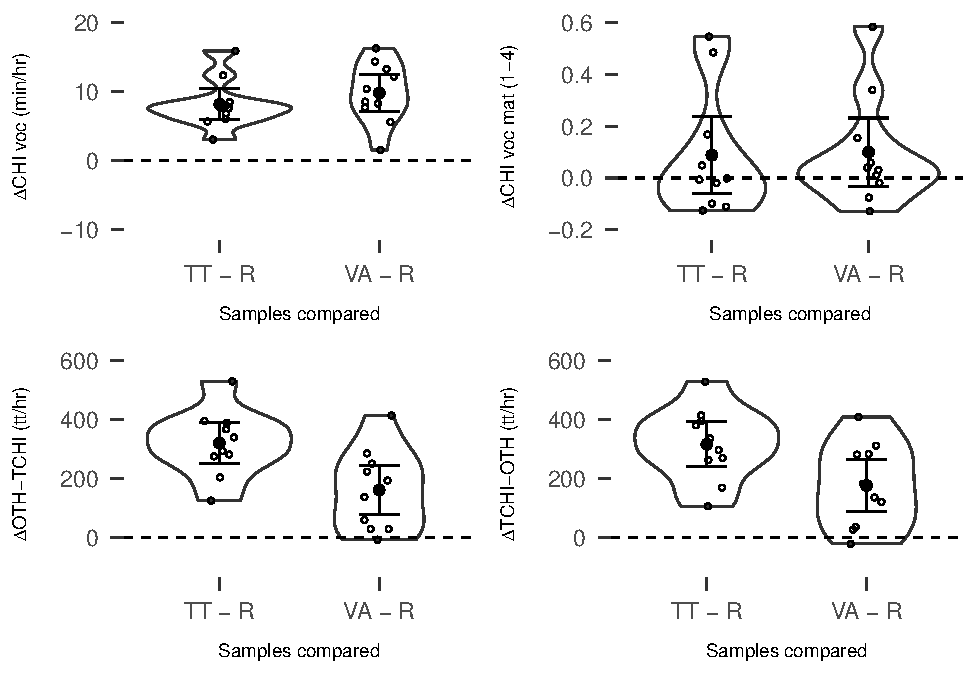
\includegraphics{Tseltal-CLE_files/figure-latex/plot_sample_differences-2.pdf}

\section{Discussion}\label{discussion}

\subsection{LATERGRAM}\label{latergram}

One serious issue is how we define adult-like linguistic competence,
especially within models in which we consider that adults still continue
learning and that individual differences are rampant between adults in
both linguistic knowledge and skill at every level, from phonetics to
syntax to pragmatics, and of course vocabulary too. When we talk about
language acquisition, especially cross-culturally, we have to be careful
about what we think the ``target'' is and what are considered to be the
developmental benchmarks children achieve. The focus recently has been
on vocabulary acquisition, for some of the reasons outline above.
However, vocabulary is a particularly literacy-centric view of language
development. If we were to go back in time and set the seed of
developmental language science in another culture, we might be much more
concerned about the acquisition of kinship systems and other complex
relational language, or in the ability to design elaborately indirect
speech acts. Acquiring a language involves the mastery of a shockingly
diverse array of skills and knowledge: not just linguistic symbols and
systems, but also the infrastructure underlying their use (e.g.,
interactional skills), the cognitive-general skills supporting those
systems. There's no reason \emph{a priori} to believe that every aspect
of language acquisition is equally influenced by environmental input.
For example, children's pointing frequency is influenced by the amount
of pointing in their environment, but the age of pointing onset---the
age which they first begin to point---appears unaffected by the
frequency of pointing in their environment (REFS: Matthews, Liszkowski).

\newpage

\section{References}\label{references}

\begingroup
\setlength{\parindent}{-0.5in} \setlength{\leftskip}{0.5in}

\hypertarget{refs}{}

\endgroup






\end{document}
